\documentclass{article}
\usepackage{tabularx}
\usepackage{longtable}
\usepackage{array}
\usepackage{float}
\usepackage{listings}
\usepackage{amsmath}
\usepackage{amssymb}
\usepackage{mathtools}
\usepackage{amsfonts}
\usepackage{graphicx}
\usepackage[table]{xcolor}
\setlength{\arrayrulewidth}{0.5mm}
\graphicspath{ {./images/} }
\usepackage[margin=20mm]{geometry}
\renewcommand{\labelenumii}{\theenumii}
\renewcommand{\theenumii}{\theenumi.\arabic{enumii}.}
\renewcommand{\arraystretch}{1.5}
\newcommand{\f}[2]{f_{#1}(#2)}
\newcommand{\code}[1]{\texttt{#1}}
\DeclarePairedDelimiter{\ceil}{\lceil}{\rceil}
\DeclarePairedDelimiter{\set}{\left\{}{\right\}}
\DeclarePairedDelimiter{\parens}{\lparen}{\rparen}
\title{HW2 Report}
\date{}
\begin{document}
\maketitle
\section*{Part 1}
\subsection*{Q1:}
    \begin{figure}[H]
        \centering
        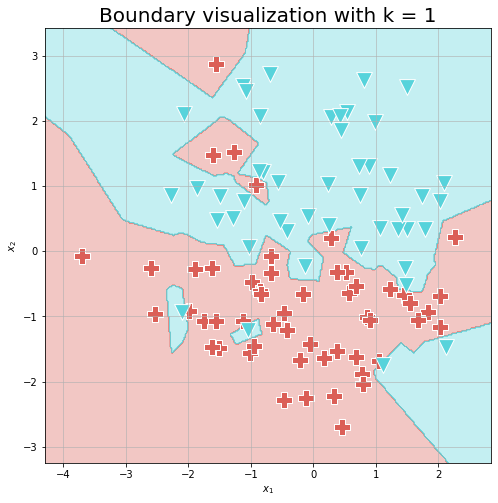
\includegraphics[scale=0.4]{q1_k1.png}
        \caption{Boundary Visualization for KNN with K = 1}
        \label{fig:q1_k1}
    \end{figure}
    \begin{figure}[H]
        \centering
        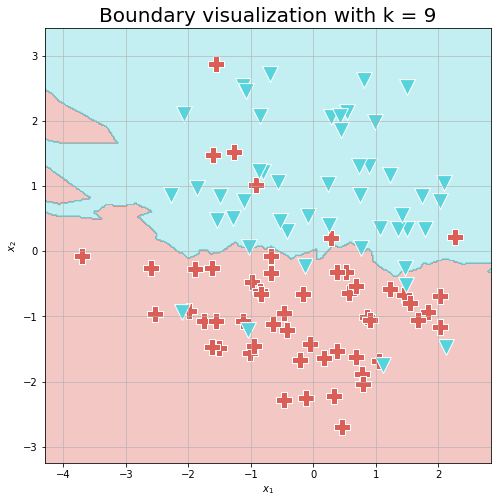
\includegraphics[scale=0.4]{q1_k9.png}
        \caption{Boundary Visualization for KNN with K = 9}
        \label{fig:q1_k9}
    \end{figure}
    \paragraph*{}
    As can be seen in figure \ref{fig:q1_k1}, the model with k equal to 1 caused overfitting to occur, as for every new sample point, its prediction took into account only the closest point to it, thereby increasing the complexity of the model since every new point is predicted locally. On the other hand, as can be seen in figure \ref{fig:q1_k9}, the model with k equal to nine takes into account the nine closest points to the sample being predicted, and therefore takes a broader outlook on the training data in-order to tdo the prediction, thereby lowering the complexity. But at the same time, we can see that a number of points were not classified correctly, and therefore this could indicate that this model is performing underfitting.
    
\subsection*{Q2:}
    \begin{figure}[H]
        \centering
        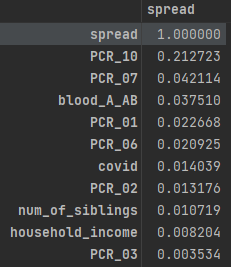
\includegraphics{images/q2.png}
        \caption{The 10 most correlated features to \code{spread}}
    \end{figure}
\subsection*{Q3:}
    \begin{figure}[H]
        \centering
        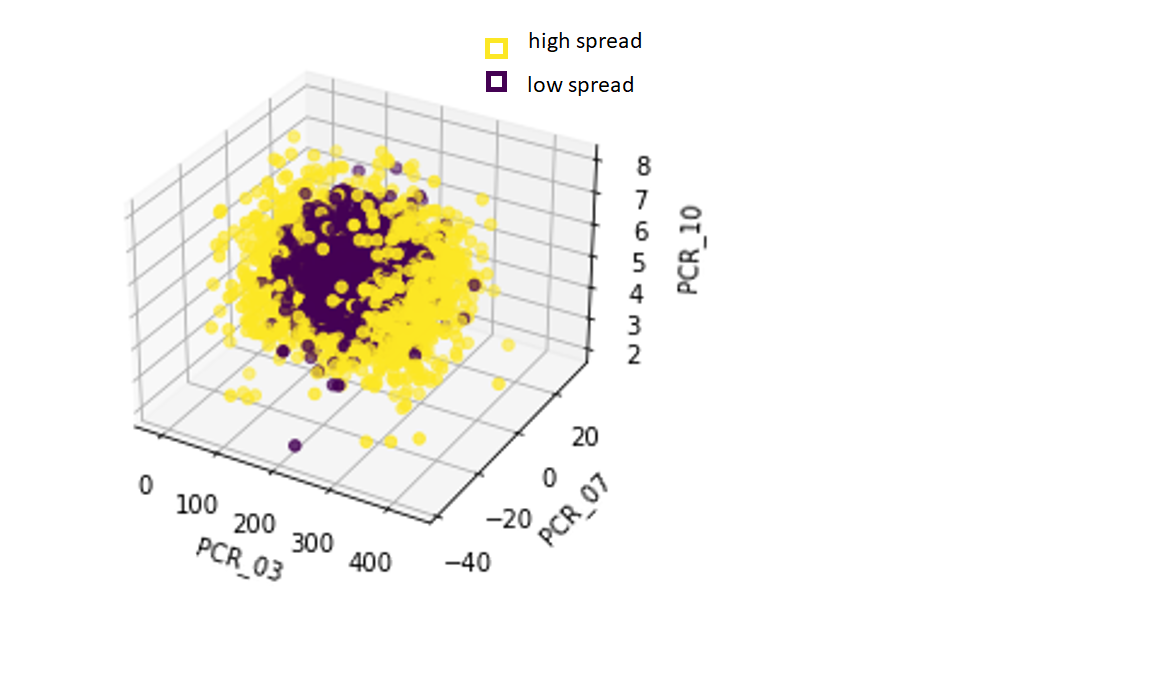
\includegraphics{images/q3.png}
        \caption{3D Scatter plot of \code{PCR\_03}, \code{PCR\_07}, and \code{PCR\_10} according to \code{spread}}
    \end{figure}
\subsection*{Q4:}
    \paragraph*{}
    The points with label -1 for \code{spread} are contained within an ellipsoid described by the following equation:
    \begin{align*}
        \frac{PCR\_03}{a^2} + \frac{PCR\_07}{b^2} + \frac{PCR\_10}{c^2} = 1
    \end{align*}
    where $a,b,c$ are positive real numbers.
\subsection*{Q5:}
    \paragraph*{}
    The training accuracy for $k=11$ is $81.333\%$.

\subsection*{Q6:}
    \paragraph*{}
    Z-score scaling scales the data of a feature by ensuring that they have zero mean and unit standard deviation, thereby causing the data to adhere to a normal distribution. Features scaled according to this technique have their outliers handled correctly, but no guarantee on the resulting range of the data is made, and the ranges of different features scaled according to Z-score may differ from each other. This technique is preferable in cases that have outliers and when the learning model assumes that the data adheres to a normal distribution . On-the-other-hand, the min-max technique involves scaling the data of a feature to a specific range (generally between 0 and 1). Contrary to the Z-score method, this technique guarantees a uniform range across features and maintains the original distribution of the data, but does not handle outliers well. Therefore, it would be preferable to use this technique only when the feature in question has no significant outliers and\_or the learning model to be used requires the feature data to fall within a certain range.
\subsection*{Q7:}
    \paragraph*{}
    The updated accuracy after normalizing the data is $88.5416\%$. This is an increase of approximately $7\%$ over the accuracy from the non-normalized data. This can be explained by the fact that KNN is an algorithm that uses euclidean distances between data points for its predictions. Therefore, it is very sensitive to differences in scales between different features, and thus features that have undergone normalization, which equalizes or nearly equalizes the scales and ranges of different features, will do better in KNN because no single feature will dominate and have more influence over other features by way of having a larger scale.  
\subsection*{Q8:}
    \begin{figure}[H]
        \centering
        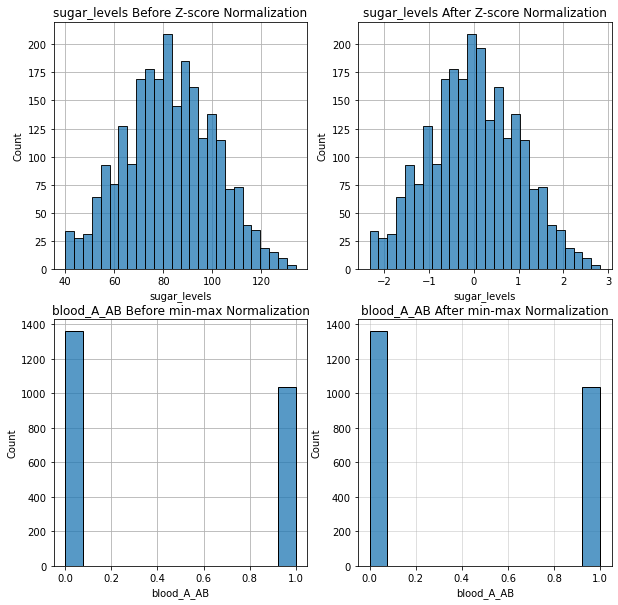
\includegraphics[scale=0.5]{q8_hists.png}
        \caption{Histogram Plots of \code{sugar\_levels} and \code{blood\_A\_AB} Before and After Normalization}
        \label{fig:q8_hist}
    \end{figure}
    \paragraph*{\code{sugar\_levels}}
    We chose to do Z-score Normalization on \code{sugar\_levels} since it already obeys an approximate normal distribution, as can be seen in figure \ref{fig:q8_hist}, and therefore we would not be forcibly changing its distribution through the normalization process. Furthermore, we will not be using it in the KNN model, which works better with  min-max normalized features, but rather with SGD SVM, which works better with Z-score normalized features, and a decision tree, which is mostly agnostic to Normalization.
    \paragraph*{\code{blood\_A\_AB}}
     In contrast, we chose to do min-max normalization on \code{blood\_A\_AB}, since it does not obey a normal distribution, but rather already obeyed a binary distribution of 0 and 1, which we did not want to modify. Furthermore, it does not have outliers which could negatively affect the min-max normalization.
\subsection*{Q9:}
    \begin{figure}[H]
        \centering
        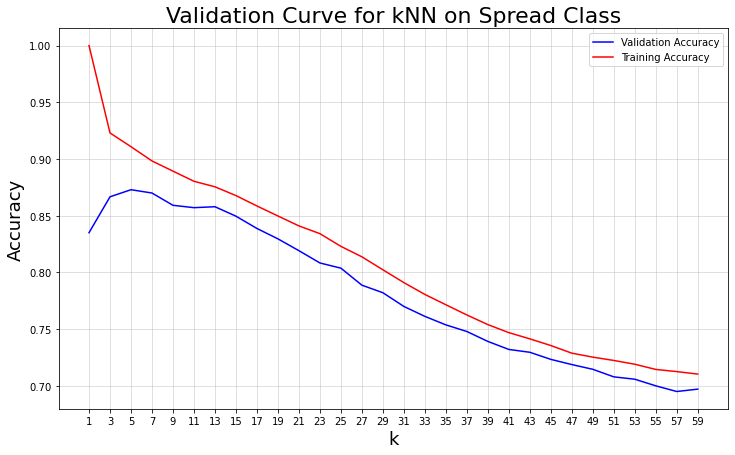
\includegraphics[scale=0.5]{q9.png}
        \caption{Validation Curve for kNN on spread Class}
        \label{fig:q9}
    \end{figure}
    \paragraph*{}
    The optimal $k$ value is 5, as can be seen by virtue of the fact that in figure \ref{fig:q9}, the highest point (peak) of the validation curve is at 5. The mean validation and training accuracies for $k=5$ are $87.2916\%$ and $91.083\%$, respectively.
\section*{Part 2}
\subsection*{Q11:}
    \begin{figure}[H]
        \centering
        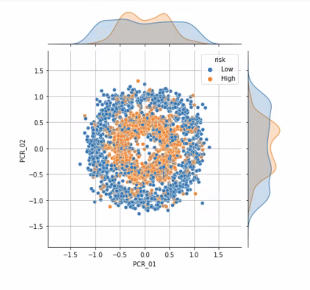
\includegraphics{q11_pcr_01_pcr_02_j_plot.png}
        \caption{Joint plot of PCR\_01 and PCR\_02 according to risk}
        \label{fig:pcr_01_pcr_02_j_plot}
    \end{figure}
    \paragraph*{}
    As can be seen from the scatter portion of the jointplot in figure \ref{fig:pcr_01_pcr_02_j_plot}, the plot is mostly separable into radiuses, and therefore it seems likely that \code{PCR\_01} and \code{PCR\_02} will be important in predicting the \code{risk} class.
    \begin{figure}[H]
        \centering
        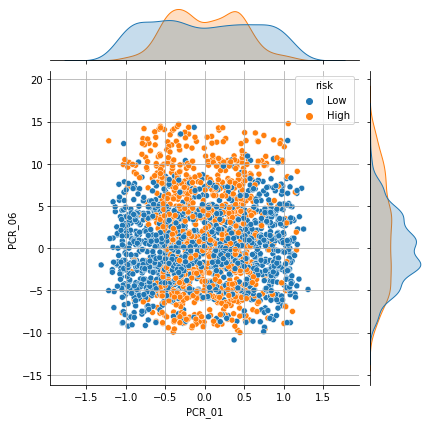
\includegraphics[scale=0.4]{q11_pcr_06_01_j_plot.png}
        \caption{Joint plot of PCR\_06 versus PCR\_01 with respect to risk}
        \label{fig:pcr_06_pcr_01_j_plot}
    \end{figure}
    \paragraph*{}
     Furthermore, from the scatter portion of the jointplot in figure \ref{fig:pcr_06_pcr_01_j_plot} we noticed a mostly separable form similar to the letter "H" where the "H" itself is made up of a high proportion of points with low risk surrounded by clusters of points of high risk. Therefore, we can conclude that in addition, \code{PCR\_06} will be important in predicting the \code{risk} class.
\subsection*{Q12:}
    \begin{figure}[H]
        \centering
        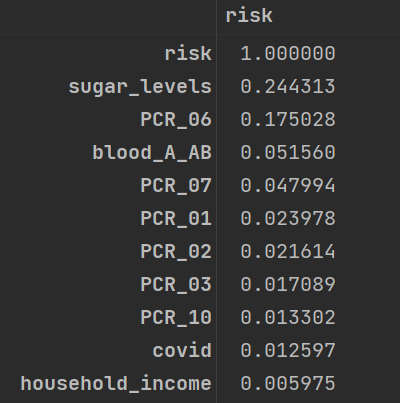
\includegraphics{images/q12.png}
        \caption{The 10 most correlated features to \code{risk}}
        \label{fig:q12}
    \end{figure}
\subsection*{Q13:}
    \begin{figure}[H]
        \centering
        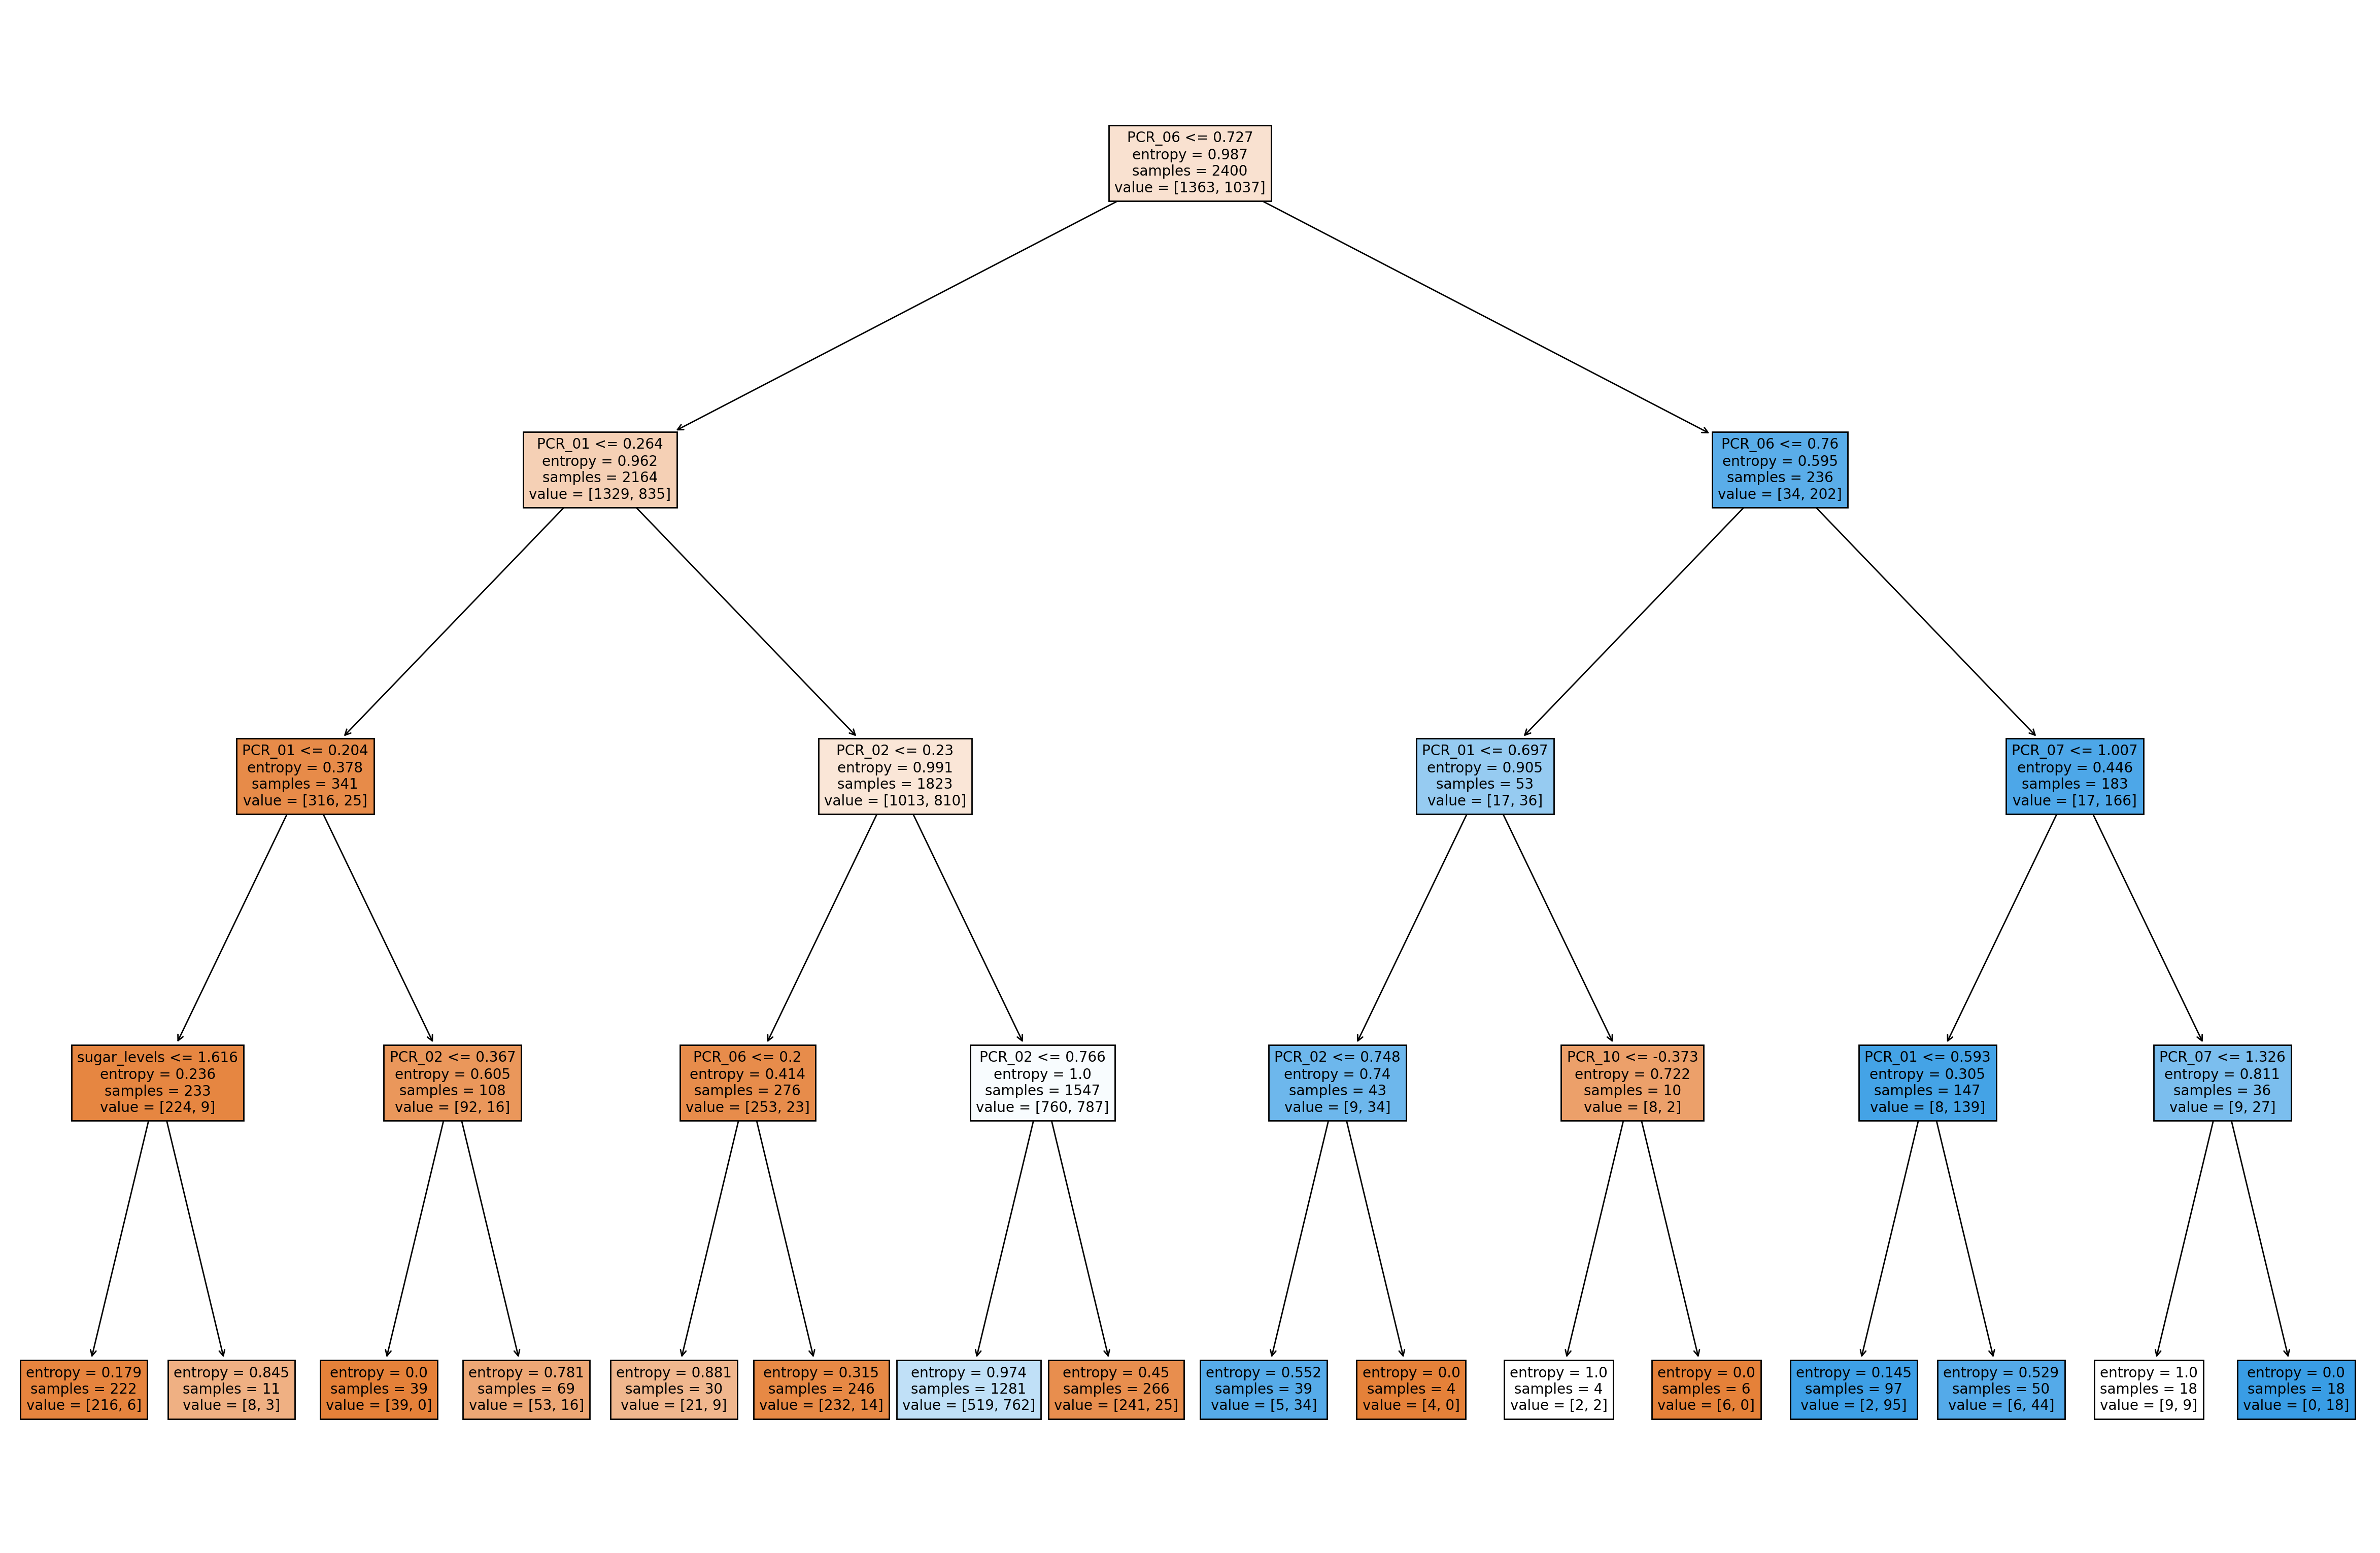
\includegraphics[scale=0.32]{q13.png}
        \caption{ID3 Decision Tree for Predicting \code{risk} CLass}
        \label{fig:q13}
    \end{figure}
    \paragraph*{}
    The training accuracy of the model is $74.333\%$.
\subsection*{Q14:}
    \paragraph*{}
    \code{PCR\_01} and \code{PCR\_02}, which we concluded would be important features, are the features with the fifth and sixth highest correlations with \code{risk}, as can be seen in figure \ref{fig:q12}, and their actual correlation values ($0.023$ and $0.021$ respectively) are very small. It is therefore easy to see that that these features are very much not discernable as important features by merely analyzing their correlation to \code{risk}. Even \code{PCR\_06}, which has the second highest correlation to \code{risk}, has a low correlation value of only $0.175$, and is therefore also not easily discernable as an important feature by way of correlation alone.
    \paragraph*{}
    All three of these features which we deemed important were used by ID3 in the decision tree. And in-fact, they were used in 11 out of 15 of the internal nodes of the tree, further proving their importance.
\subsection*{Q15:}
    \begin{figure}[H]
        \centering
        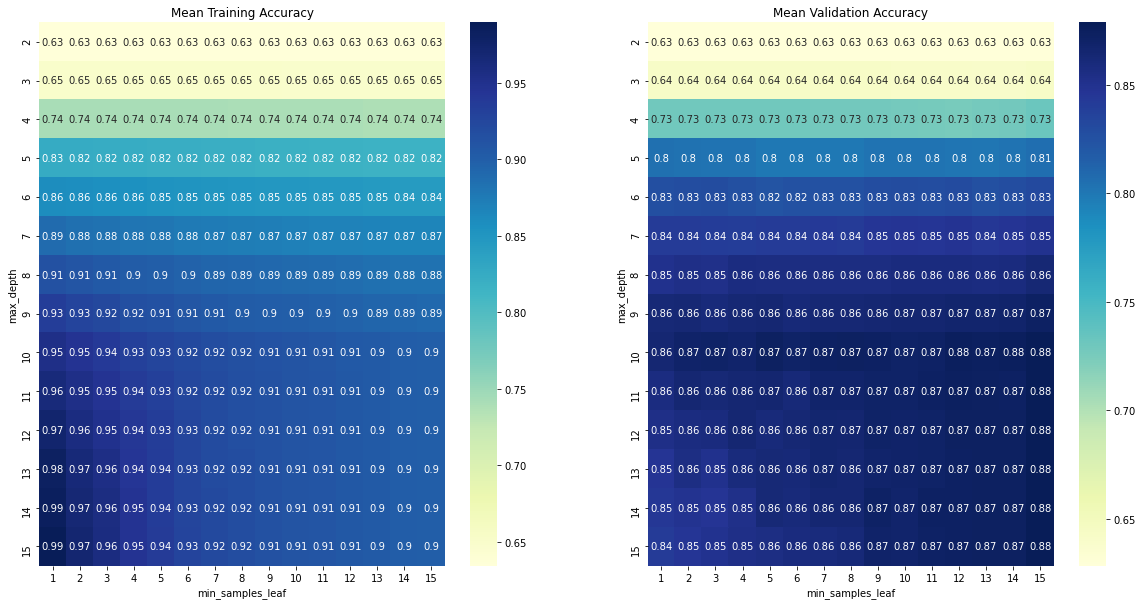
\includegraphics[scale=0.48]{q15.png}
        \caption{Heat Maps of Training and Validation Accuracies of ID3 on \code{risk} Class for Different Values of \code{max\_depth} and \code{min\_samples\_leaf} Hyper-Parameters}
        \label{fig:q15}
    \end{figure}
    \paragraph*{}
    The optimal hyperparameter combination is a \code{max\_depth}=10 and \code{min\_samples\_leaf}=15, since they produce the highest validation accuracy of $88\%$ with the minimal required depth and highest minimum sample leaf requirement, as can be seen in the mean validation accuracy heat map in figure \ref{fig:q15}.
    \paragraph*{}
    The combination of \code{max\_depth}=2 and \code{min\_samples\_leaf}=1 causes underfitting, as this leads to a low training accuracy of $63\%$.
    \paragraph*{}
    The combination of \code{max\_depth}=15 and \code{min\_samples\_leaf}=1 causes overfitting, as this leads to a high training accuracy of $99\%$ versus a relatively low validation accuracy of $84\%$.
\section*{Part 3}
\subsection*{Q20:}
    \paragraph*{}
    In Q19, we used a 2 dimensional polynomial transform on the features within the primal objective of the SVM model. This approach is slower than the two dimensional kernel objective because it involves computing inner products between data points and the $w$ vector in high dimensions, whereas in the kernel case, the dual objective is used, which only involves computing the kernel function for 2 dimensional polynomials which is of much lower dimension (and finding and storing the $\alpha$s, which is not too computationally burdensome on the assumption that the support vectors are sparse).



\end{document}